% Created by tikzDevice version 0.12.3 on 2019-09-27 15:30:16
% !TEX encoding = UTF-8 Unicode
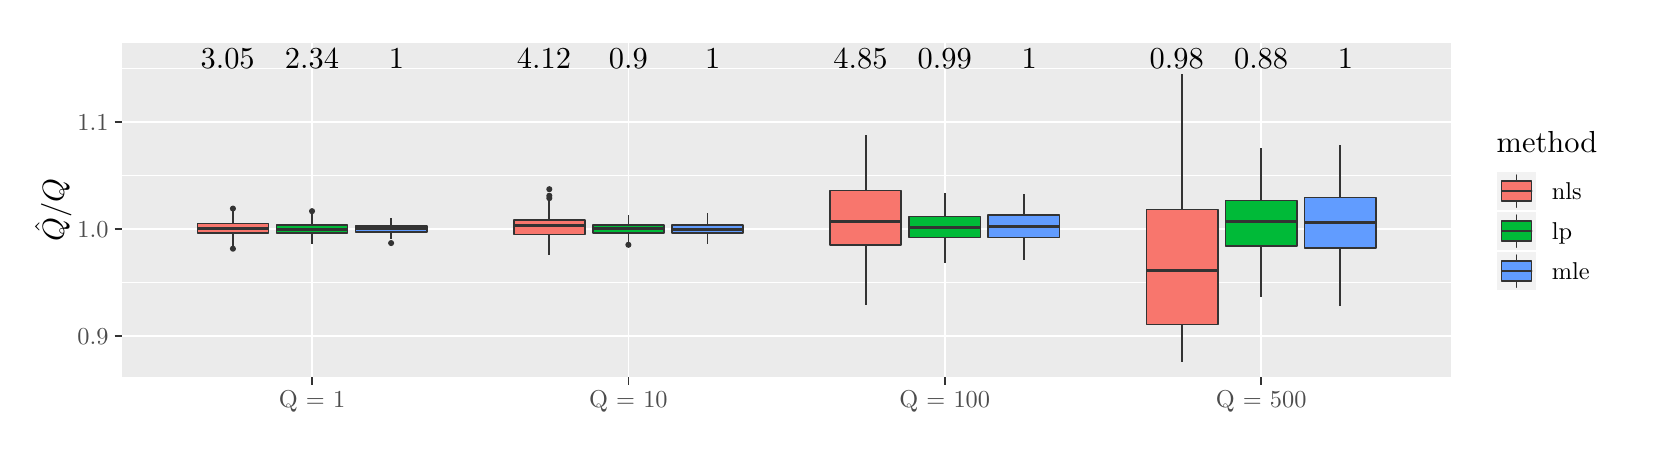
\begin{tikzpicture}[x=1pt,y=1pt]
\definecolor{fillColor}{RGB}{255,255,255}
\path[use as bounding box,fill=fillColor,fill opacity=0.00] (0,0) rectangle (578.16,144.54);
\begin{scope}
\path[clip] (  0.00,  0.00) rectangle (578.16,144.54);
\definecolor{drawColor}{RGB}{255,255,255}
\definecolor{fillColor}{RGB}{255,255,255}

\path[draw=drawColor,line width= 0.6pt,line join=round,line cap=round,fill=fillColor] (  0.00,  0.00) rectangle (578.16,144.54);
\end{scope}
\begin{scope}
\path[clip] ( 34.16, 18.22) rectangle (514.31,139.04);
\definecolor{fillColor}{gray}{0.92}

\path[fill=fillColor] ( 34.16, 18.22) rectangle (514.31,139.04);
\definecolor{drawColor}{RGB}{255,255,255}

\path[draw=drawColor,line width= 0.3pt,line join=round] ( 34.16, 52.50) --
	(514.31, 52.50);

\path[draw=drawColor,line width= 0.3pt,line join=round] ( 34.16, 91.09) --
	(514.31, 91.09);

\path[draw=drawColor,line width= 0.3pt,line join=round] ( 34.16,129.68) --
	(514.31,129.68);

\path[draw=drawColor,line width= 0.6pt,line join=round] ( 34.16, 33.21) --
	(514.31, 33.21);

\path[draw=drawColor,line width= 0.6pt,line join=round] ( 34.16, 71.80) --
	(514.31, 71.80);

\path[draw=drawColor,line width= 0.6pt,line join=round] ( 34.16,110.38) --
	(514.31,110.38);

\path[draw=drawColor,line width= 0.6pt,line join=round] (102.75, 18.22) --
	(102.75,139.04);

\path[draw=drawColor,line width= 0.6pt,line join=round] (217.07, 18.22) --
	(217.07,139.04);

\path[draw=drawColor,line width= 0.6pt,line join=round] (331.39, 18.22) --
	(331.39,139.04);

\path[draw=drawColor,line width= 0.6pt,line join=round] (445.71, 18.22) --
	(445.71,139.04);
\definecolor{drawColor}{gray}{0.20}
\definecolor{fillColor}{gray}{0.20}

\path[draw=drawColor,line width= 0.4pt,line join=round,line cap=round,fill=fillColor] ( 74.17, 79.17) circle (  0.89);

\path[draw=drawColor,line width= 0.4pt,line join=round,line cap=round,fill=fillColor] ( 74.17, 64.67) circle (  0.89);

\path[draw=drawColor,line width= 0.6pt,line join=round] ( 74.17, 73.77) -- ( 74.17, 78.34);

\path[draw=drawColor,line width= 0.6pt,line join=round] ( 74.17, 70.36) -- ( 74.17, 65.74);
\definecolor{fillColor}{RGB}{248,118,109}

\path[draw=drawColor,line width= 0.6pt,line join=round,line cap=round,fill=fillColor] ( 61.31, 73.77) --
	( 61.31, 70.36) --
	( 87.03, 70.36) --
	( 87.03, 73.77) --
	( 61.31, 73.77) --
	cycle;

\path[draw=drawColor,line width= 1.1pt,line join=round] ( 61.31, 71.87) -- ( 87.03, 71.87);
\definecolor{fillColor}{gray}{0.20}

\path[draw=drawColor,line width= 0.4pt,line join=round,line cap=round,fill=fillColor] (102.75, 78.23) circle (  0.89);

\path[draw=drawColor,line width= 0.6pt,line join=round] (102.75, 73.13) -- (102.75, 77.03);

\path[draw=drawColor,line width= 0.6pt,line join=round] (102.75, 70.26) -- (102.75, 66.20);
\definecolor{fillColor}{RGB}{0,186,56}

\path[draw=drawColor,line width= 0.6pt,line join=round,line cap=round,fill=fillColor] ( 89.89, 73.13) --
	( 89.89, 70.26) --
	(115.61, 70.26) --
	(115.61, 73.13) --
	( 89.89, 73.13) --
	cycle;

\path[draw=drawColor,line width= 1.1pt,line join=round] ( 89.89, 71.68) -- (115.61, 71.68);
\definecolor{fillColor}{gray}{0.20}

\path[draw=drawColor,line width= 0.4pt,line join=round,line cap=round,fill=fillColor] (131.33, 66.70) circle (  0.89);

\path[draw=drawColor,line width= 0.6pt,line join=round] (131.33, 72.78) -- (131.33, 75.66);

\path[draw=drawColor,line width= 0.6pt,line join=round] (131.33, 70.75) -- (131.33, 68.32);
\definecolor{fillColor}{RGB}{97,156,255}

\path[draw=drawColor,line width= 0.6pt,line join=round,line cap=round,fill=fillColor] (118.47, 72.78) --
	(118.47, 70.75) --
	(144.19, 70.75) --
	(144.19, 72.78) --
	(118.47, 72.78) --
	cycle;

\path[draw=drawColor,line width= 1.1pt,line join=round] (118.47, 71.80) -- (144.19, 71.80);
\definecolor{fillColor}{gray}{0.20}

\path[draw=drawColor,line width= 0.4pt,line join=round,line cap=round,fill=fillColor] (188.49, 83.81) circle (  0.89);

\path[draw=drawColor,line width= 0.4pt,line join=round,line cap=round,fill=fillColor] (188.49, 82.94) circle (  0.89);

\path[draw=drawColor,line width= 0.4pt,line join=round,line cap=round,fill=fillColor] (188.49, 86.17) circle (  0.89);

\path[draw=drawColor,line width= 0.6pt,line join=round] (188.49, 74.98) -- (188.49, 82.04);

\path[draw=drawColor,line width= 0.6pt,line join=round] (188.49, 69.86) -- (188.49, 62.54);
\definecolor{fillColor}{RGB}{248,118,109}

\path[draw=drawColor,line width= 0.6pt,line join=round,line cap=round,fill=fillColor] (175.63, 74.98) --
	(175.63, 69.86) --
	(201.35, 69.86) --
	(201.35, 74.98) --
	(175.63, 74.98) --
	cycle;

\path[draw=drawColor,line width= 1.1pt,line join=round] (175.63, 73.09) -- (201.35, 73.09);
\definecolor{fillColor}{gray}{0.20}

\path[draw=drawColor,line width= 0.4pt,line join=round,line cap=round,fill=fillColor] (217.07, 66.08) circle (  0.89);

\path[draw=drawColor,line width= 0.6pt,line join=round] (217.07, 73.24) -- (217.07, 76.81);

\path[draw=drawColor,line width= 0.6pt,line join=round] (217.07, 70.41) -- (217.07, 67.22);
\definecolor{fillColor}{RGB}{0,186,56}

\path[draw=drawColor,line width= 0.6pt,line join=round,line cap=round,fill=fillColor] (204.21, 73.24) --
	(204.21, 70.41) --
	(229.93, 70.41) --
	(229.93, 73.24) --
	(204.21, 73.24) --
	cycle;

\path[draw=drawColor,line width= 1.1pt,line join=round] (204.21, 71.96) -- (229.93, 71.96);

\path[draw=drawColor,line width= 0.6pt,line join=round] (245.65, 73.23) -- (245.65, 77.70);

\path[draw=drawColor,line width= 0.6pt,line join=round] (245.65, 70.24) -- (245.65, 66.29);
\definecolor{fillColor}{RGB}{97,156,255}

\path[draw=drawColor,line width= 0.6pt,line join=round,line cap=round,fill=fillColor] (232.79, 73.23) --
	(232.79, 70.24) --
	(258.51, 70.24) --
	(258.51, 73.23) --
	(232.79, 73.23) --
	cycle;

\path[draw=drawColor,line width= 1.1pt,line join=round] (232.79, 71.72) -- (258.51, 71.72);

\path[draw=drawColor,line width= 0.6pt,line join=round] (302.81, 85.76) -- (302.81,105.91);

\path[draw=drawColor,line width= 0.6pt,line join=round] (302.81, 66.11) -- (302.81, 44.50);
\definecolor{fillColor}{RGB}{248,118,109}

\path[draw=drawColor,line width= 0.6pt,line join=round,line cap=round,fill=fillColor] (289.95, 85.76) --
	(289.95, 66.11) --
	(315.67, 66.11) --
	(315.67, 85.76) --
	(289.95, 85.76) --
	cycle;

\path[draw=drawColor,line width= 1.1pt,line join=round] (289.95, 74.52) -- (315.67, 74.52);

\path[draw=drawColor,line width= 0.6pt,line join=round] (331.39, 76.36) -- (331.39, 84.74);

\path[draw=drawColor,line width= 0.6pt,line join=round] (331.39, 68.73) -- (331.39, 59.43);
\definecolor{fillColor}{RGB}{0,186,56}

\path[draw=drawColor,line width= 0.6pt,line join=round,line cap=round,fill=fillColor] (318.53, 76.36) --
	(318.53, 68.73) --
	(344.25, 68.73) --
	(344.25, 76.36) --
	(318.53, 76.36) --
	cycle;

\path[draw=drawColor,line width= 1.1pt,line join=round] (318.53, 72.29) -- (344.25, 72.29);

\path[draw=drawColor,line width= 0.6pt,line join=round] (359.97, 76.88) -- (359.97, 84.46);

\path[draw=drawColor,line width= 0.6pt,line join=round] (359.97, 68.69) -- (359.97, 60.65);
\definecolor{fillColor}{RGB}{97,156,255}

\path[draw=drawColor,line width= 0.6pt,line join=round,line cap=round,fill=fillColor] (347.11, 76.88) --
	(347.11, 68.69) --
	(372.83, 68.69) --
	(372.83, 76.88) --
	(347.11, 76.88) --
	cycle;

\path[draw=drawColor,line width= 1.1pt,line join=round] (347.11, 72.53) -- (372.83, 72.53);

\path[draw=drawColor,line width= 0.6pt,line join=round] (417.13, 78.84) -- (417.13,127.93);

\path[draw=drawColor,line width= 0.6pt,line join=round] (417.13, 37.33) -- (417.13, 23.71);
\definecolor{fillColor}{RGB}{248,118,109}

\path[draw=drawColor,line width= 0.6pt,line join=round,line cap=round,fill=fillColor] (404.27, 78.84) --
	(404.27, 37.33) --
	(430.00, 37.33) --
	(430.00, 78.84) --
	(404.27, 78.84) --
	cycle;

\path[draw=drawColor,line width= 1.1pt,line join=round] (404.27, 56.76) -- (430.00, 56.76);

\path[draw=drawColor,line width= 0.6pt,line join=round] (445.71, 82.04) -- (445.71,101.19);

\path[draw=drawColor,line width= 0.6pt,line join=round] (445.71, 65.64) -- (445.71, 47.37);
\definecolor{fillColor}{RGB}{0,186,56}

\path[draw=drawColor,line width= 0.6pt,line join=round,line cap=round,fill=fillColor] (432.85, 82.04) --
	(432.85, 65.64) --
	(458.58, 65.64) --
	(458.58, 82.04) --
	(432.85, 82.04) --
	cycle;

\path[draw=drawColor,line width= 1.1pt,line join=round] (432.85, 74.56) -- (458.58, 74.56);

\path[draw=drawColor,line width= 0.6pt,line join=round] (474.29, 83.15) -- (474.29,102.11);

\path[draw=drawColor,line width= 0.6pt,line join=round] (474.29, 65.02) -- (474.29, 44.11);
\definecolor{fillColor}{RGB}{97,156,255}

\path[draw=drawColor,line width= 0.6pt,line join=round,line cap=round,fill=fillColor] (461.43, 83.15) --
	(461.43, 65.02) --
	(487.16, 65.02) --
	(487.16, 83.15) --
	(461.43, 83.15) --
	cycle;

\path[draw=drawColor,line width= 1.1pt,line join=round] (461.43, 74.30) -- (487.16, 74.30);
\definecolor{drawColor}{RGB}{0,0,0}

\node[text=drawColor,anchor=base,inner sep=0pt, outer sep=0pt, scale=  1.10] at (133.23,129.75) {1};

\node[text=drawColor,anchor=base,inner sep=0pt, outer sep=0pt, scale=  1.10] at (102.75,129.75) {2.34};

\node[text=drawColor,anchor=base,inner sep=0pt, outer sep=0pt, scale=  1.10] at ( 72.26,129.75) {3.05};

\node[text=drawColor,anchor=base,inner sep=0pt, outer sep=0pt, scale=  1.10] at (247.56,129.75) {1};

\node[text=drawColor,anchor=base,inner sep=0pt, outer sep=0pt, scale=  1.10] at (217.07,129.75) {0.9};

\node[text=drawColor,anchor=base,inner sep=0pt, outer sep=0pt, scale=  1.10] at (186.59,129.75) {4.12};

\node[text=drawColor,anchor=base,inner sep=0pt, outer sep=0pt, scale=  1.10] at (361.88,129.75) {1};

\node[text=drawColor,anchor=base,inner sep=0pt, outer sep=0pt, scale=  1.10] at (331.39,129.75) {0.99};

\node[text=drawColor,anchor=base,inner sep=0pt, outer sep=0pt, scale=  1.10] at (300.91,129.75) {4.85};

\node[text=drawColor,anchor=base,inner sep=0pt, outer sep=0pt, scale=  1.10] at (476.20,129.75) {1};

\node[text=drawColor,anchor=base,inner sep=0pt, outer sep=0pt, scale=  1.10] at (445.71,129.75) {0.88};

\node[text=drawColor,anchor=base,inner sep=0pt, outer sep=0pt, scale=  1.10] at (415.23,129.75) {0.98};
\end{scope}
\begin{scope}
\path[clip] (  0.00,  0.00) rectangle (578.16,144.54);
\definecolor{drawColor}{gray}{0.30}

\node[text=drawColor,anchor=base east,inner sep=0pt, outer sep=0pt, scale=  0.88] at ( 29.21, 30.18) {0.9};

\node[text=drawColor,anchor=base east,inner sep=0pt, outer sep=0pt, scale=  0.88] at ( 29.21, 68.77) {1.0};

\node[text=drawColor,anchor=base east,inner sep=0pt, outer sep=0pt, scale=  0.88] at ( 29.21,107.35) {1.1};
\end{scope}
\begin{scope}
\path[clip] (  0.00,  0.00) rectangle (578.16,144.54);
\definecolor{drawColor}{gray}{0.20}

\path[draw=drawColor,line width= 0.6pt,line join=round] ( 31.41, 33.21) --
	( 34.16, 33.21);

\path[draw=drawColor,line width= 0.6pt,line join=round] ( 31.41, 71.80) --
	( 34.16, 71.80);

\path[draw=drawColor,line width= 0.6pt,line join=round] ( 31.41,110.38) --
	( 34.16,110.38);
\end{scope}
\begin{scope}
\path[clip] (  0.00,  0.00) rectangle (578.16,144.54);
\definecolor{drawColor}{gray}{0.20}

\path[draw=drawColor,line width= 0.6pt,line join=round] (102.75, 15.47) --
	(102.75, 18.22);

\path[draw=drawColor,line width= 0.6pt,line join=round] (217.07, 15.47) --
	(217.07, 18.22);

\path[draw=drawColor,line width= 0.6pt,line join=round] (331.39, 15.47) --
	(331.39, 18.22);

\path[draw=drawColor,line width= 0.6pt,line join=round] (445.71, 15.47) --
	(445.71, 18.22);
\end{scope}
\begin{scope}
\path[clip] (  0.00,  0.00) rectangle (578.16,144.54);
\definecolor{drawColor}{gray}{0.30}

\node[text=drawColor,anchor=base,inner sep=0pt, outer sep=0pt, scale=  0.88] at (102.75,  7.21) {Q = 1};

\node[text=drawColor,anchor=base,inner sep=0pt, outer sep=0pt, scale=  0.88] at (217.07,  7.21) {Q = 10};

\node[text=drawColor,anchor=base,inner sep=0pt, outer sep=0pt, scale=  0.88] at (331.39,  7.21) {Q = 100};

\node[text=drawColor,anchor=base,inner sep=0pt, outer sep=0pt, scale=  0.88] at (445.71,  7.21) {Q = 500};
\end{scope}
\begin{scope}
\path[clip] (  0.00,  0.00) rectangle (578.16,144.54);
\definecolor{drawColor}{RGB}{0,0,0}

\node[text=drawColor,rotate= 90.00,anchor=base,inner sep=0pt, outer sep=0pt, scale=  1.10] at ( 13.08, 78.63) {$\hat{Q}/Q$};
\end{scope}
\begin{scope}
\path[clip] (  0.00,  0.00) rectangle (578.16,144.54);
\definecolor{fillColor}{RGB}{255,255,255}

\path[fill=fillColor] (525.31, 43.84) rectangle (572.66,113.42);
\end{scope}
\begin{scope}
\path[clip] (  0.00,  0.00) rectangle (578.16,144.54);
\definecolor{drawColor}{RGB}{0,0,0}

\node[text=drawColor,anchor=base west,inner sep=0pt, outer sep=0pt, scale=  1.10] at (530.81, 99.27) {method};
\end{scope}
\begin{scope}
\path[clip] (  0.00,  0.00) rectangle (578.16,144.54);
\definecolor{drawColor}{RGB}{255,255,255}
\definecolor{fillColor}{gray}{0.95}

\path[draw=drawColor,line width= 0.6pt,line join=round,line cap=round,fill=fillColor] (530.81, 78.25) rectangle (545.26, 92.70);
\end{scope}
\begin{scope}
\path[clip] (  0.00,  0.00) rectangle (578.16,144.54);
\definecolor{drawColor}{gray}{0.20}

\path[draw=drawColor,line width= 0.6pt,line join=round,line cap=round] (538.03, 79.70) --
	(538.03, 81.86);

\path[draw=drawColor,line width= 0.6pt,line join=round,line cap=round] (538.03, 89.09) --
	(538.03, 91.26);
\definecolor{fillColor}{RGB}{248,118,109}

\path[draw=drawColor,line width= 0.6pt,line join=round,line cap=round,fill=fillColor] (532.61, 81.86) rectangle (543.45, 89.09);

\path[draw=drawColor,line width= 0.6pt,line join=round,line cap=round] (532.61, 85.48) --
	(543.45, 85.48);
\end{scope}
\begin{scope}
\path[clip] (  0.00,  0.00) rectangle (578.16,144.54);
\definecolor{drawColor}{RGB}{255,255,255}
\definecolor{fillColor}{gray}{0.95}

\path[draw=drawColor,line width= 0.6pt,line join=round,line cap=round,fill=fillColor] (530.81, 63.80) rectangle (545.26, 78.25);
\end{scope}
\begin{scope}
\path[clip] (  0.00,  0.00) rectangle (578.16,144.54);
\definecolor{drawColor}{gray}{0.20}

\path[draw=drawColor,line width= 0.6pt,line join=round,line cap=round] (538.03, 65.24) --
	(538.03, 67.41);

\path[draw=drawColor,line width= 0.6pt,line join=round,line cap=round] (538.03, 74.64) --
	(538.03, 76.81);
\definecolor{fillColor}{RGB}{0,186,56}

\path[draw=drawColor,line width= 0.6pt,line join=round,line cap=round,fill=fillColor] (532.61, 67.41) rectangle (543.45, 74.64);

\path[draw=drawColor,line width= 0.6pt,line join=round,line cap=round] (532.61, 71.02) --
	(543.45, 71.02);
\end{scope}
\begin{scope}
\path[clip] (  0.00,  0.00) rectangle (578.16,144.54);
\definecolor{drawColor}{RGB}{255,255,255}
\definecolor{fillColor}{gray}{0.95}

\path[draw=drawColor,line width= 0.6pt,line join=round,line cap=round,fill=fillColor] (530.81, 49.34) rectangle (545.26, 63.80);
\end{scope}
\begin{scope}
\path[clip] (  0.00,  0.00) rectangle (578.16,144.54);
\definecolor{drawColor}{gray}{0.20}

\path[draw=drawColor,line width= 0.6pt,line join=round,line cap=round] (538.03, 50.79) --
	(538.03, 52.96);

\path[draw=drawColor,line width= 0.6pt,line join=round,line cap=round] (538.03, 60.18) --
	(538.03, 62.35);
\definecolor{fillColor}{RGB}{97,156,255}

\path[draw=drawColor,line width= 0.6pt,line join=round,line cap=round,fill=fillColor] (532.61, 52.96) rectangle (543.45, 60.18);

\path[draw=drawColor,line width= 0.6pt,line join=round,line cap=round] (532.61, 56.57) --
	(543.45, 56.57);
\end{scope}
\begin{scope}
\path[clip] (  0.00,  0.00) rectangle (578.16,144.54);
\definecolor{drawColor}{RGB}{0,0,0}

\node[text=drawColor,anchor=base west,inner sep=0pt, outer sep=0pt, scale=  0.88] at (550.76, 82.45) {nls};
\end{scope}
\begin{scope}
\path[clip] (  0.00,  0.00) rectangle (578.16,144.54);
\definecolor{drawColor}{RGB}{0,0,0}

\node[text=drawColor,anchor=base west,inner sep=0pt, outer sep=0pt, scale=  0.88] at (550.76, 67.99) {lp};
\end{scope}
\begin{scope}
\path[clip] (  0.00,  0.00) rectangle (578.16,144.54);
\definecolor{drawColor}{RGB}{0,0,0}

\node[text=drawColor,anchor=base west,inner sep=0pt, outer sep=0pt, scale=  0.88] at (550.76, 53.54) {mle};
\end{scope}
\end{tikzpicture}
